\addtocontents{toc}{\vspace{\baselineskip}\noindent{\titlefont\bfseries\large I\quad Background}\par\vspace{0.3em}}
\chapter{MicroRTS as a Sequential Decision Problem}
\label{chap:background}

This chapter introduces the MicroRTS environment and formalizes it as a sequential decision-making problem. The chapter first situates MicroRTS within the broader context of real-time strategy games and identifies the algorithmic challenges they pose for Artificial Intelligence, then describes the MicroRTS environment in detail and casts the resulting problem as a Markov Decision Process under full observability. The notations and abstractions introduced here form the common foundation upon which all subsequent chapters build.

\section{Real-Time Strategy Games}
\label{sec:rts}

\subsection{Genre Overview}

RTS games are competitive video games\footnote{Not to be confused with Multiplayer Online Battle Arena (MOBA) games such as 
\href{https://www.leagueoflegends.com}{League of Legends} (Riot Games, 2009) or \href{https://www.dota2.com}{Dota~2} (Valve Corporation, 2013), which restrict each player to a single hero rather than full army and economy management.} in which two or more players simultaneously gather resources, construct bases, and command armies~\cite{ontanonSurveyRealTimeStrategy2013}. Unlike turn-based games, decisions unfold in real time, forcing players to manage their economy, coordinate heterogeneous units, and react to opponent actions simultaneously. Skilled play requires both \emph{macro-management} (economy, production, and build orders) and \emph{micro-management} (individual unit positioning and combat control). Figure~\ref{fig:rts-games} shows three well-known examples of the genre.

\begin{figure}[!ht]
    \centering
    \begin{subfigure}{0.34\textwidth}
        \centering
        
\includegraphics[width=\linewidth]{chapters/02_microrts_decision_problem/figures/starcraft2.pdf}
        \caption{
            \centering
            \urlref{https://starcraft2.blizzard.com}{StarCraft II}
        }
    \end{subfigure}
    \hfill
    \begin{subfigure}{0.31\textwidth}
        \centering
        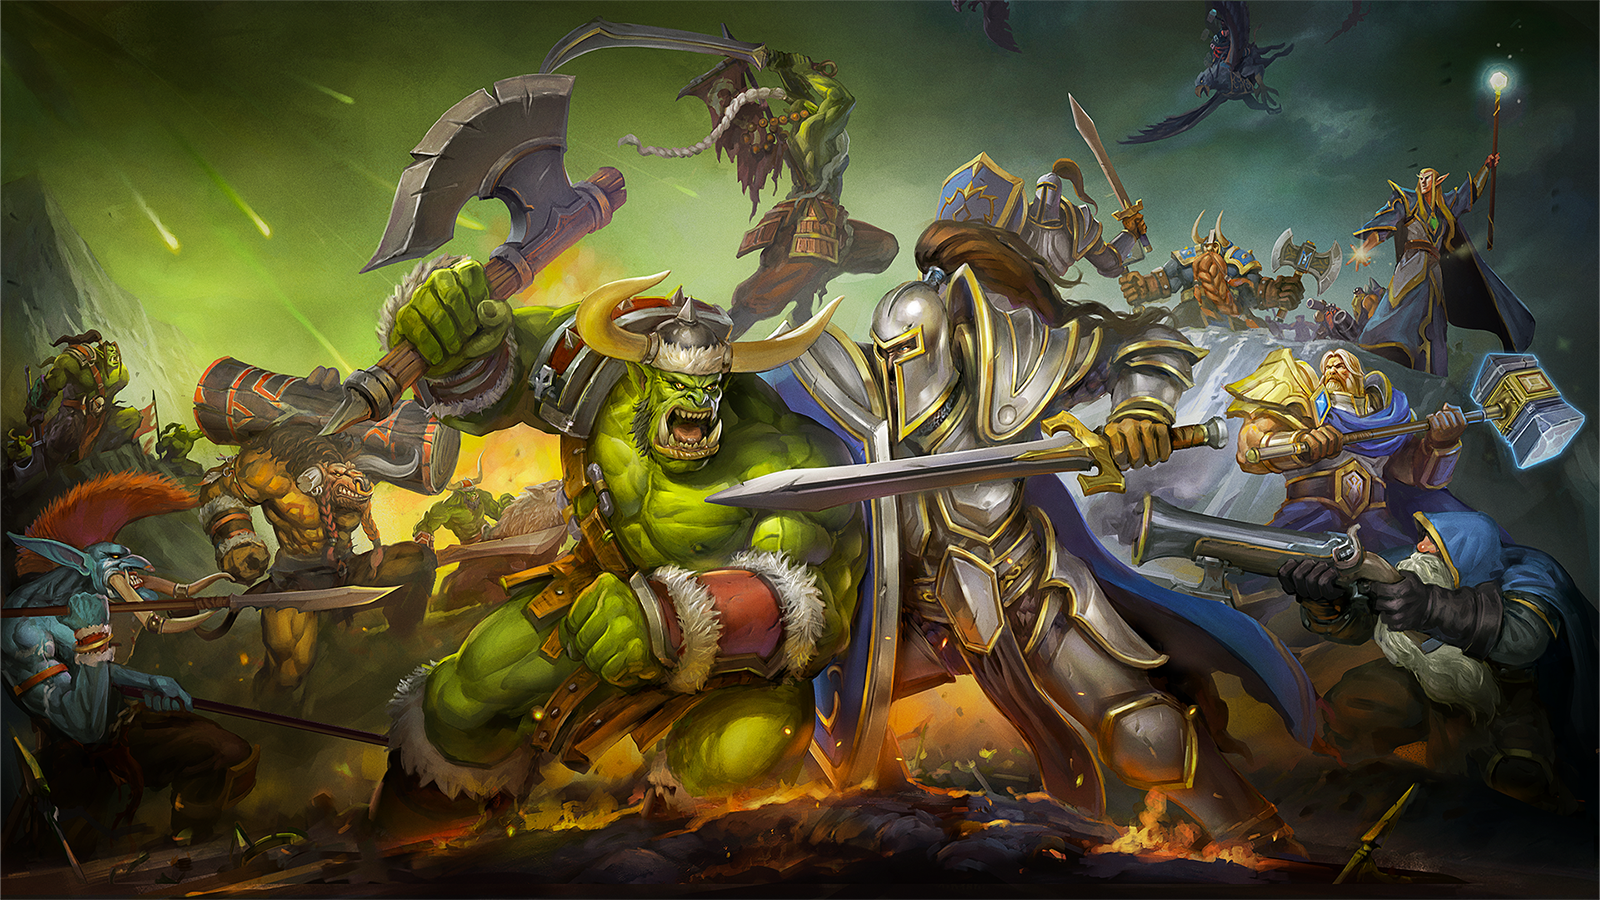
\includegraphics[width=\linewidth]{chapters/02_microrts_decision_problem/figures/warcraft3.png}
        \caption{
            \centering
            \urlref{https://warcraft3.blizzard.com}{Warcraft III}
        }
    \end{subfigure}
    \hfill
    \begin{subfigure}{0.31\textwidth}
        \centering
        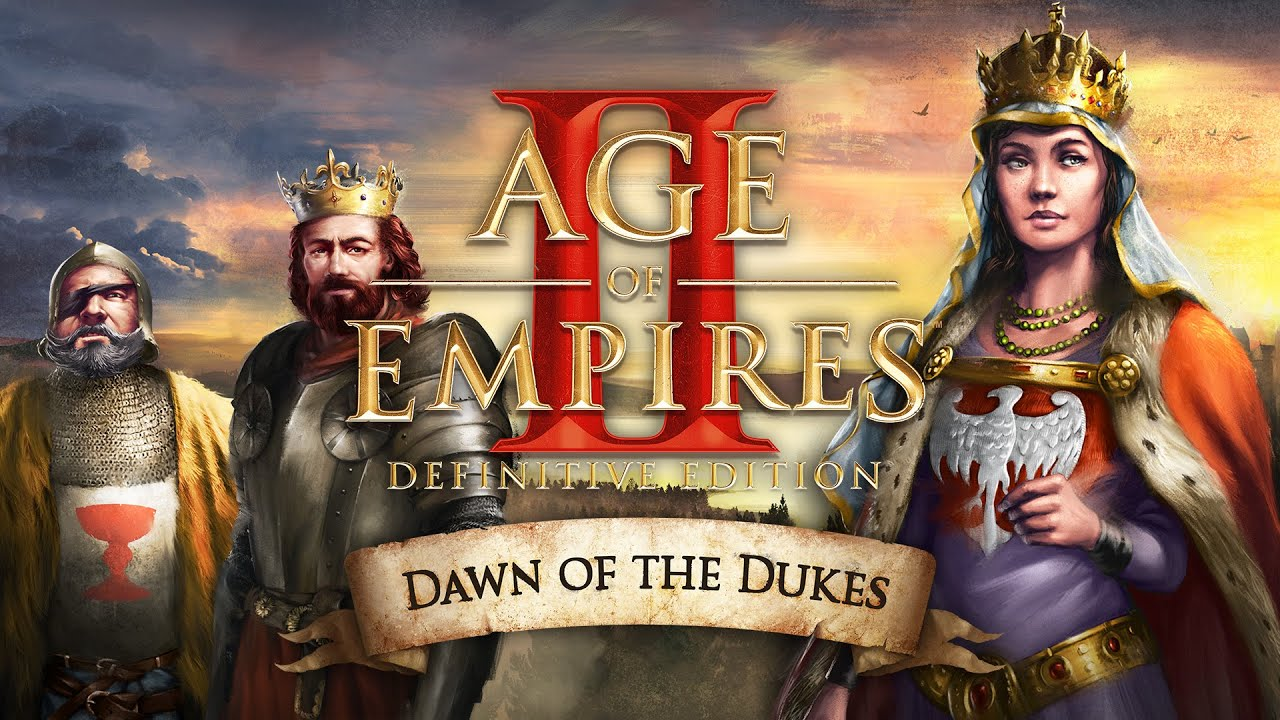
\includegraphics[width=\linewidth]{chapters/02_microrts_decision_problem/figures/AgeOfEmpire.jpg}
        \caption{
        \centering
        \urlref{https://www.ageofempires.com/games/aoeiide/}{Age of Empires II}
        }
    \end{subfigure}
    \caption[Three well-known RTS games]{Three well-known RTS games. Images from Blizzard Entertainment (2010, 2002) and World's Edge \& Xbox Game Studios (2019).}
    \label{fig:rts-games}
\end{figure}

\subsection{AI Research Challenges}

RTS games pose several well-identified challenges for AI~\cite{buroRTSChallenge2003, ontanonSurveyRealTimeStrategy2013}. First, the joint action space grows combinatorially with the number of units on the field. Second, decisions are made under real-time constraints, leaving no room for exhaustive deliberation. Third, games last thousands of timesteps with a sparse terminal reward signal (win, loss, or draw) providing no intermediate feedback. Fourth, the opponent adapts continuously, making the environment non-stationary from a single agent's perspective. Finally, skilled play requires both macro-management and micro-management simultaneously, forcing the agent to make decisions at multiple temporal scales. These challenges are addressed progressively throughout Chapters~\ref{chap:background}--\ref{chap:sota}.

\section{MicroRTS Environment}
\label{sec:microrts_env}

Commercial RTS games such as StarCraft~II have served as prominent benchmarks for RL research~\cite{vinyalsStarCraftIINew2017}, but their scale precludes controlled experimentation, as illustrated by AlphaStar~\cite{vinyalsGrandmasterLevelStarCraft2019}, whose training demanded prohibitive computational resources to interface with the game.

MicroRTS\footnote{S. Ontañón, MicroRTS, 2012, GitHub: \url{https://github.com/Farama-Foundation/MicroRTS}.} avoids these costs by providing a minimalist RTS environment designed for AI research~\cite{ontanonCombinatorialMultiArmedBandit2013}. Built on a Java engine, it uses small grid-based maps and retains the core RTS mechanics (resource gathering, base building, army control) with simplified movement and reduced unit diversity. The environment also supports optional fog-of-war\footnote{Fog-of-war is a visibility mechanic where units can only see within a limited radius, concealing the rest of the map.} and stochastic damage\footnote{Stochastic damage adds a random multiplier to attack damage; disabled by default to keep transitions deterministic given fixed actions.}~\cite{richouxMicroPhantomPlayingMicroRTS2020, antuoriConstrainedOptimizationUncertainty2019}, though neither is used in this thesis. This reduced complexity makes experiments faster and more reproducible, while the combinatorial action space and simultaneous unit control keep the problem challenging. Figure~\ref{fig:microrts-screenshot} illustrates the main elements of the MicroRTS simulator interface.

\begin{figure}[!ht]
    \centering
    \begin{minipage}[c]{0.5\columnwidth}
        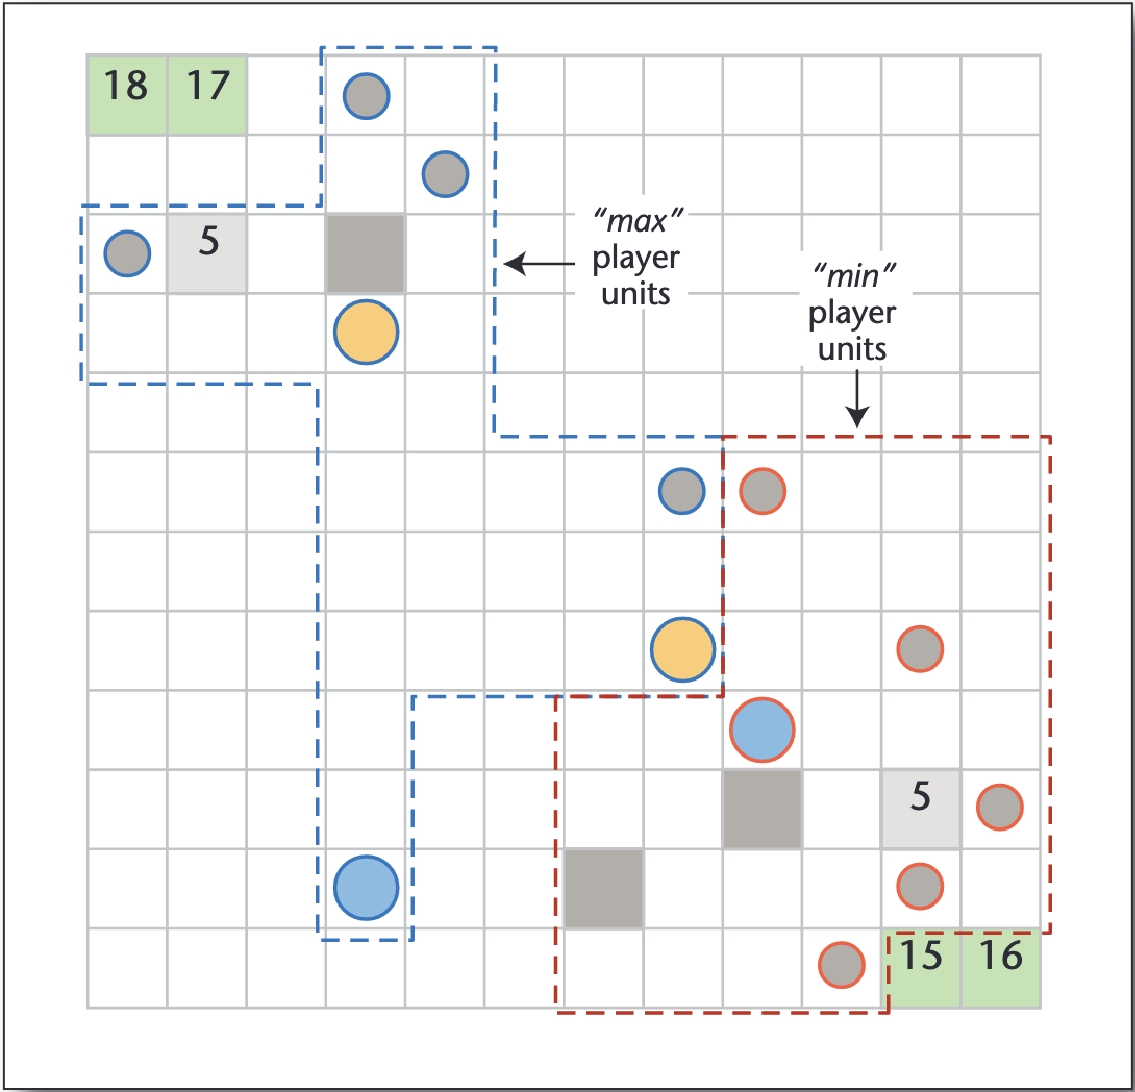
\includegraphics[width=\linewidth]{chapters/02_microrts_decision_problem/figures/microRTS-image.pdf}
    \end{minipage}
    \hfill
    \begin{minipage}[c]{0.45\columnwidth}
        \captionof{figure}[Typical MicroRTS game state]{
            Typical game state on a $12{\times}12$ grid map. Square entities denote bases (light gray), barracks (dark gray), and resource mines (green); circular units represent workers (small) and military units (large). Numbers on resource mines indicate remaining stock; numbers on bases indicate the player's current resources. Blue units belong to the \emph{max player}, red to the \emph{min player}~\cite{ontanonFirstMicroRTSArtificial2018}.
        }
        \label{fig:microrts-screenshot}
    \end{minipage}
\end{figure}

\subsection{Annual AI Competition}
\label{subsec:competition}

MicroRTS has been supported by an annual AI competition since $2017$\footnote{S. Ontañón, MicroRTS AI competition, Google Sites: \url{https://sites.google.com/site/micrortsaicompetition/}.}, hosted at various IEEE conferences (CIG, CoG, and WCCI, the World Congress on Computational Intelligence). The evaluation benchmark assembled in Chapter~\ref{chap:evaluation-framework} draws on the open-source winners of these competition editions. Figure~\ref{fig:microrts-competition-timeline} summarizes the competition timeline.

\begin{figure}[!ht]
\centering
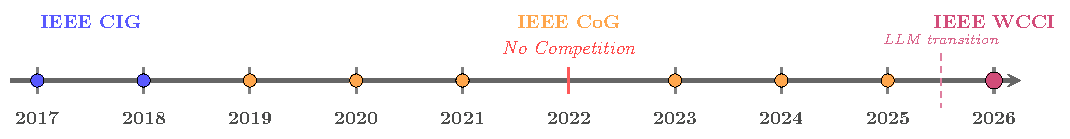
\includegraphics[width=\linewidth]{chapters/02_microrts_decision_problem/figures/microrts_timeline.pdf}
\caption[MicroRTS competition timeline ($2017$--$2026$)]{Timeline of the MicroRTS competition ($2017$--$2026$) showing hosting conferences.}
\label{fig:microrts-competition-timeline}
\end{figure}

The $2026$ edition marks a shift toward evaluating LLMs as game-playing agents\footnote{Official $2026$ MicroRTS competition description: \url{https://github.com/drchangliu/MicroRTS/blob/master/COMPETITION.md}.}~\cite{cuiEmpoweringLLMsParameterized2025, maAdaptiveCommandRealTime2025}, a direction orthogonal to this thesis. Since no RL-focused edition is available, a tournament framework is developed in Chapter~\ref{chap:evaluation-framework} to reproduce the $2023$ competition format as closely as possible, enabling fair and reliable comparison against past competition winners.

\subsection{Formal Game State}
\label{sec:format-game-state}

MicroRTS environments are defined over discrete two-dimensional grid maps\footnote{The formalization presented in this section is derived from analysis of the MicroRTS source code and game documentation.}.

Let $H, W \in \mathbb{N}_0$\footnote{This work uses the convention $\mathbb{N} = \{0, 1, 2, \ldots\}$ and $\mathbb{N}_0 = \{1, 2, 3, \ldots\}$.} denote the map height and width, respectively. The set of valid cell coordinates is:
\begin{align}
\mathcal{G} = \{0, \dots, W-1\} \times \{0, \dots, H-1\} \subset \mathbb{N}^2.
\end{align}
The terrain layout is described by a binary map:
\begin{align}
\mathcal{M}: \mathcal{G} \to \{0, 1\}, \quad (x,y) \mapsto 
\begin{cases} 
1 & \text{if cell } (x,y) \text{ is passable,} \\ 
0 & \text{if cell } (x,y) \text{ is a terrain obstacle.}
\end{cases}
\end{align}
Since $\mathcal{M}$ is fixed throughout a game, it is treated as a game parameter rather than part of the dynamic state.
At any timestep $t$, the complete game state is defined as the tuple:
\begin{align}
\boldsymbol{s}_t =
\bigl(
    \tau_t,\;
    \boldsymbol{\rho}_t,\;
    \mathcal{U}_t
\bigr),
\label{eq:tuple_state}
\end{align}
where $\tau_t \in \llbracket 0, T_{\max} \rrbracket$\footnote{$\llbracket a, b \rrbracket$ denotes the set of integers $\{a, a+1, \ldots, b\}$ for $a, b \in \mathbb{Z}$.} is the current simulation timestep, $\boldsymbol{\rho}_t = (\rho_t^1, \rho_t^2) \in \mathbb{N}^2$ the accumulated resource count for each player, and $\mathcal{U}_t = \{\mathbf{u}^{t}_1, \dots, \mathbf{u}^{t}_{n_t}\}$ the set of $n_t$ entities present on the map.

Each entity $\mathbf{u}^{t}_i \in \mathcal{U}_t$ is characterized by the tuple:
\begin{align}
\mathbf{u}^{t}_i = 
\bigl(
    \mathrm{player}_i,\; \mathbf{pos}^{t}_i,\; 
    \mathrm{type}_i,\; 
    \mathrm{hp}^{t}_i,\; \mathrm{res}^{t}_i,\; \mathbf{action}^{t}_i
\bigr),
\end{align}
where the components are defined as follows:
\begin{itemize}
    \item $\mathrm{player}_i \in \{p_1, p_2, \text{neutral}\}$: entity ownership;
    \item $\mathbf{pos}^{t}_i \in \mathcal{G}$: grid position;
    \item $\mathrm{type}_i \in \mathcal{K} = \{\text{Resource}, \text{Base}, \text{Barracks}, \text{Worker}, \text{Light}, \text{Heavy}, \text{Ranged}\}$: entity type;
    \item $\mathrm{hp}^{t}_i \in \llbracket 0, \mathrm{HP}_{\max}(\mathrm{type}_i) \rrbracket$: current hit points (HP);
    \item $\mathrm{res}^{t}_i \in \mathbb{N}$: carried resources for Workers ($0$ or $1$), remaining stock for Resource nodes ($\in \llbracket 0, \mathrm{res}_{\max}^{i} \rrbracket$), and $0$ for all others;
    \item $\mathbf{action}^{t}_i = (\mathrm{action\_type}^{t}_i,\; \boldsymbol{\varphi}^{t}_i, \mathrm{timer}^{t}_i)$: action being executed, where $\mathrm{action\_type}^{t}_i \in \mathcal{A}_{\text{type}} = \\ \{\text{None}, \text{Move}, \text{Harvest}, \text{Return}, \text{Produce}, \text{Attack}\}$, parameters $\boldsymbol{\varphi}^{t}_i$ (Table~\ref{tab:microrts-action-details}), and $\mathrm{timer}^{t}_i$ the remaining steps before completion.
\end{itemize}

The entity set $\mathcal{U}_t$ evolves over time: it grows when a \emph{Produce} action completes, spawning a new unit or creating a new structure, and it shrinks when an entity's hit points reach zero through combat damage or when a Resource node is fully depleted by harvesting. In both cases the entity does not appear in $\mathcal{U}_{t+1}$ and its cell becomes unoccupied.

\subsection{Unit Types and Combat}
\label{sec:microrts-units}

Each entity type in $\mathcal{K}$ fulfills a distinct strategic role. Their quantitative attributes are summarized in Table~\ref{tab:microrts-units}, available actions in Table~\ref{tab:microrts-actions}, and action details in Table~\ref{tab:microrts-action-details}.

\begin{table}[!htp]
\centering
\small

% ============ Table 1 ============
\caption[Unit attributes and combat parameters in MicroRTS]{Unit attributes and combat parameters in MicroRTS.\footnotemark}
\label{tab:microrts-units}
\begin{tabularx}{\textwidth}{Xcccccccc}
\toprule
\textbf{Unit Type} & \textbf{Production} & \textbf{Production} & \textbf{Hit} & \textbf{Move} & \textbf{Attack} & \textbf{Attack} & \textbf{Attack} \\
 & \textbf{Cost} & \textbf{Time} & \textbf{Points} & \textbf{Time} & \textbf{Time} & \textbf{Damage} & \textbf{Range} \\
\midrule
\multicolumn{8}{l}{\textit{Static entities}} \\
\midrule
Resource\textsuperscript{$\dagger$} & — & — & — & — & — & — & — \\
Base & $10$ & $250$ & $10$ & — & — & — & — \\
Barracks & $5$ & $200$ & $4$ & — & — & — & — \\
\midrule
\multicolumn{8}{l}{\textit{Mobile units}} \\
\midrule
Worker\textsuperscript{$\ddagger$} & $1$ & $50$ & $1$ & $10$ & $5$ & $1$ & $1$ \\
Light & $2$ & $80$ & $4$ & $8$ & $5$ & $2$ & $1$ \\
Heavy & $2$ & $120$ & $4$ & $12$ & $5$ & $4$ & $1$ \\
Ranged & $2$ & $100$ & $1$ & $10$ & $5$ & $1$ & $3$ \\
\bottomrule
\multicolumn{8}{p{\textwidth}}{\footnotesize 
    \textsuperscript{$\dagger$}Resource nodes have no combat or production role; their only attribute is the remaining resource stock. \newline
    \textsuperscript{$\ddagger$}Workers also perform Harvest ($20$ steps) and Return ($10$ steps) actions; see Table~\ref{tab:microrts-action-details}.} \\
\end{tabularx}

\vspace{3em}

% ============ Table 2 ============
\caption[Action availability by unit type]{Action availability by unit type in MicroRTS.\textsuperscript{\ref{fn:microrts-wiki}}}
\label{tab:microrts-actions}
\begin{tabularx}{\textwidth}{Xccccccc}
\toprule
\textbf{Unit Type} & \textbf{None} & \textbf{Move} & \textbf{Attack} & \textbf{Harvest} & \textbf{Return} & \textbf{Produce} & $\boldsymbol{|\mathcal{A}_i|^{\dagger}}$ \\
\midrule
\multicolumn{8}{l}{\textit{Static entities}} \\
\midrule
Resource  & \checkmark & — & — & — & — & — & $1$ \\
Base      & \checkmark & — & — & — & — & \checkmark & $5$ \\
Barracks  & \checkmark & — & — & — & — & \checkmark & $13$ \\
\midrule
\multicolumn{8}{l}{\textit{Mobile units}} \\
\midrule
Worker & \checkmark & \checkmark & \checkmark & \checkmark & \checkmark & \checkmark & $70$ \\
Light  & \checkmark & \checkmark & \checkmark & — & — & — & $54$ \\
Heavy  & \checkmark & \checkmark & \checkmark & — & — & — & $54$ \\
Ranged & \checkmark & \checkmark & \checkmark & — & — & — & $54$ \\
\bottomrule
\multicolumn{8}{p{\textwidth}}{\footnotesize
    Checkmarks (\checkmark) indicate available actions; dashes (—) indicate unavailable actions.\newline
    \textsuperscript{$\dagger$}\,$|\mathcal{A}_i|$ is the API-level (Application Programming Interface) syntactic cardinality discussed in Section~\ref{subsec:microrts_mdp}; runtime feasibility is enforced by an invalid-action mask.} \\
\end{tabularx}

\vspace{3em}

% ============ Table 3 ============
\caption[Action parameters and execution details]{Action parameters $\boldsymbol{\varphi}$ and execution details in MicroRTS.\textsuperscript{\ref{fn:microrts-wiki}}}
\label{tab:microrts-action-details}
\begin{tabularx}{\textwidth}{llX}
\toprule
\textbf{Action} & \textbf{Parameters} & \textbf{Notes} \\
\midrule
None & Duration & Unit idles for specified time. \\
\midrule
Move & Direction\textsuperscript{†} & Move one cell in specified direction. Fails if blocked or occupied. \\
\midrule
Attack & Target (x, y) & Melee range $1$, Ranged range $3$. Damage applied on final cycle only. \\
\midrule
Harvest & Direction\textsuperscript{†} & Collect $1$ resource from adjacent node. Worker only, empty inventory. \\
\midrule
Return & Direction\textsuperscript{†} & Deposit carried resource to adjacent Base. Worker only, full inventory. \\
\midrule
Produce & Direction\textsuperscript{†}, Type\textsuperscript{‡} & Base produces Workers; Barracks produces Light, Heavy, or Ranged; Worker constructs Base or Barracks. Requires resources. \\
\bottomrule
\multicolumn{3}{p{\textwidth}}{\footnotesize \textsuperscript{†}Direction $\in \mathcal{D} = \{\uparrow, \rightarrow, \downarrow, \leftarrow\}$ \quad | \quad \textsuperscript{‡}Type $\in \mathcal{K} \setminus \{\text{Resource}\}$} \\
\end{tabularx}

\end{table}
\footnotetext{Farama Foundation, MicroRTS game definition, $2018$, GitHub Wiki: \url{https://github.com/Farama-Foundation/MicroRTS/wiki/Game-Definition}.\label{fn:microrts-wiki}}

\paragraph*{Resources} are static and neutral; they are the only source of income. Each resource node contains a finite stock that can be harvested by Workers and deposited at Bases.

\paragraph*{Buildings} are static, player-owned structures that define production capabilities. Bases enable Worker production and accept resource deposits. Barracks unlock military production (Light, Heavy, and Ranged units). Neither building can attack.

\paragraph*{Mobile units} perform all active tasks: resource collection, construction, and combat. Workers are the only units that can harvest, return resources, and construct buildings, but their 1~HP makes them fragile and vulnerable to any attack. They can still attack at melee range with low damage, enabling early-game worker rushes. The three military types form a rock-paper-scissors cycle (Figure~\ref{fig:unit-counters}): Light counters Ranged through superior mobility, Ranged counters Heavy by attacking from distance, and Heavy counters Light with high damage. This cyclic dominance forces players to mix unit compositions rather than mass-produce one type.

\vspace{-0.5em}

\begin{figure}[!ht]
    \centering
    \begin{minipage}[c]{0.5\columnwidth}
        \centering
        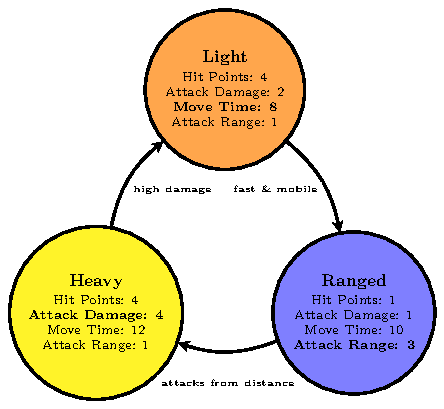
\includegraphics[width=\linewidth]{chapters/02_microrts_decision_problem/figures/unit_counters.pdf}
    \end{minipage}
    \hfill
    \begin{minipage}[c]{0.45\columnwidth}
        \captionof{figure}[Unit type relationships (rock-paper-scissors)]{
            Unit type relationships in MicroRTS (rock-paper-scissors cycle): Light beats Ranged thanks to faster movement, Ranged beats Heavy by dealing damage from outside melee range, and Heavy beats Light by dealing fatal damage in one hit. Colors match the in-game units, and bold marks each unit's dominant attribute.
        }
        \label{fig:unit-counters}
    \end{minipage}
\end{figure}

\vspace{-0.5em}

\subsection{Specific Game Rules}
\label{sec:action-constraints}

\paragraph*{Action execution.} Once issued, an action runs to completion; new commands are accepted only when the unit is idle. Any idle unit without a valid command defaults to a \emph{None} action.

\vspace{-0.2em}

\paragraph*{Combat.} Attacks depend only on Euclidean distance\footnote{For two grid positions $(x_1, y_1), (x_2, y_2) \in \mathcal{G}$, the Euclidean distance is $d(\mathbf{p}_1, \mathbf{p}_2) = \sqrt{(x_1-x_2)^2 + (y_1-y_2)^2}$. A unit at $\mathbf{p}_1$ can attack a target at $\mathbf{p}_2$ if and only if $d(\mathbf{p}_1, \mathbf{p}_2) \leq r$, where $r$ is the unit's attack range.}, so ranged units can fire through walls and other entities.

\vspace{-0.2em}

\paragraph*{Victory.} A player wins by eliminating all entities in $\mathcal{U}_t$ owned by the opponent while retaining at least one entity of their own (any structure or mobile unit). The game ends in a draw if both players lose their last entities on the same step, or if $\tau_t$ reaches the time limit $T_{\max}$ (commonly $3\,000$ to $8\,000$ steps); in the latter case, entity counts and resource stocks are not used as tie-breakers.

\subsection{MicroRTS-Py: Python Interface}

While MicroRTS is implemented in Java, most RL research relies on Python frameworks such as \emph{PyTorch}~\cite{paszkePyTorchImperativeStyle2019} and \emph{Stable-Baselines3}~\cite{raffinStableBaselines3ReliableReinforcement}. The MicroRTS-Py\footnote{C. Huang, MicroRTS-Py, 2019. GitHub: \url{https://github.com/Farama-Foundation/MicroRTS-Py}.} (formerly Gym-$\mu$RTS) wrapper~\cite{huangGym$m$RTSAffordableFull2021} bridges this gap via \emph{JPype}\footnote{JPype Project, Jpype – a Python to Java bridge, 2025. GitHub: \url{https://github.com/jpype-project/jpype}.} with a \emph{Gymnasium}-compatible~\cite{towersGymnasiumStandardInterface2025} Python interface to the MicroRTS engine, exposing observations, action spaces, and reward signals usable by standard RL training loops. This wrapper provides the foundation of the environment stack used in this thesis, extended with custom environments and training wrappers 
(Chapter~\ref{chap:python_bridge}).

\section{Mathematical Formulation of MicroRTS}
\label{sec:mdp_formulation}

This section formalizes MicroRTS as a sequential decision-making problem, providing a common foundation for the classical planning methods, search-based approaches, and reinforcement learning algorithms developed in subsequent chapters.

\subsection{From Markov Game to POMDP / MDP}
\label{sec:MDP}

RTS games involve $N \geq 2$ competing players. MicroRTS focuses on the 1v1 setting; the underlying problem is therefore formally a \emph{two-player zero-sum\footnote{A two-player game is \emph{zero-sum} when one player's gain is exactly the other's loss. In MicroRTS, this holds for the terminal win/loss reward.} simultaneous-move Markov game}~\cite{littmanMarkovGamesFramework1994}, where players commit to actions at each tick without observing the opponent's choice.

In this thesis, the opponent's actions are absorbed into the transition function $\mathcal{T}$, reducing the problem to a single-agent perspective. For a fixed opponent policy, this induces a stationary single-agent MDP. However, when the opponent changes across training (e.g., curriculum learning or self-play), $\mathcal{T}$ shifts with it, creating non-stationarity. Additionally, a stochastic opponent policy makes $\mathcal{T}$ stochastic from the agent's perspective, even though the underlying engine is deterministic.

\medskip

For generality, the formulation is first presented with fog-of-war enabled, in which case the problem is a \emph{Partially Observable Markov Decision Process} (POMDP)~\cite{kaelblingPlanningActingPartially1998, suttonReinforcementLearningIntroduction2020}, defined by the tuple:
\begin{align}
\langle \mathcal{S}, \mathcal{A}, \mathcal{T}, \mathcal{R}, \boldsymbol{\Omega}, \mathcal{O}, \gamma \rangle,
\label{eq:tuple_POMDP}
\end{align}
where:
\begin{itemize}
    \item $\mathcal{S}$ is the state space, encompassing all game configurations;
    \item $\mathcal{A}$ is the agent's action space;
    \item $\mathcal{T}: \mathcal{S} \times \mathcal{A} \to \Delta(\mathcal{S})$\footnote{$\Delta(\mathcal{X})$ is the set of probability distributions over $\mathcal{X}$.} is the state transition function;
    \item $\mathcal{R}: \mathcal{S} \times \mathcal{A} \times \mathcal{S} \to \mathbb{R}$ is the reward function;
    \item $\boldsymbol{\Omega}$ is the observation space;
    \item $\mathcal{O}: \mathcal{S} \times \mathcal{A} \to \Delta(\boldsymbol{\Omega})$ is the observation function;
    \item $\gamma \in [0,1)$ is the discount factor.
\end{itemize}

The discount factor $\gamma$ sets the agent's effective planning horizon: $\gamma = 0$ makes the agent myopic (only immediate rewards matter), while $\gamma$ close to $1$ lets rewards far into the future still meaningfully influence current decisions.

\medskip

Since all experiments in this thesis use full observability, $\mathcal{O}$ is the identity mapping and $\boldsymbol{\Omega} = \mathcal{S}$, so the observation components of~\ref{eq:tuple_POMDP} drop out. The POMDP reduces to a \emph{Markov Decision Process}~\cite{putermanMarkovDecisionProcesses1994}, defined by the simplified tuple:
\begin{align}
\langle \mathcal{S}, \mathcal{A}, \mathcal{T}, \mathcal{R}, \gamma \rangle.
\label{eq:tuple_MDP}
\end{align}
The MDP formulation rests on the \emph{Markov property}, which also underlies the \emph{Markov game} and the \emph{POMDP}'s latent state: the next state depends only on the current state and action, not on the history. MicroRTS satisfies this at the level of the full engine state; whether a given \emph{observation} encoding preserves it is a separate question, revisited in Chapter~\ref{chap:python_bridge} when discussing temporal memory.

\subsection{MicroRTS as an MDP}
\label{subsec:microrts_mdp}

Each component of the MDP tuple is now instantiated for MicroRTS, using the formal game state notation introduced in Section~\ref{sec:format-game-state}. The concrete implementation choices (observation encoding, action space factorization, and reward components) are detailed in Chapter~\ref{chap:python_bridge}.

\subsubsection{State Space}

Each state $\boldsymbol{s}_t \in \mathcal{S}$ corresponds to the tuple of~\ref{eq:tuple_state}: clock, per-player resources, and the entity set with attributes. For a fixed map, $\mathcal{S}$ is finite but combinatorially large: even a coarse upper bound on a $16{\times}16$ map exceeds $10^{300}$ distinct configurations\footnote{Each of the 256 cells of a $16\times16$ map admits 15 occupancy states (empty, obstacle, resource, or one of 6 player-owned entity types $\times$ 2 owners), yielding $\sim 15^{256} \approx 10^{301}$ raw configurations before per-entity attributes (HP, timers, carried resources). This is an upper bound on syntactic configurations; game constraints (limited resources, production costs) make most unreachable in practice.}, far beyond explicit enumeration. Most of the algorithms used in this thesis therefore operate on compact representations of the state.

\subsubsection{Action Space}

At each decision step, the agent issues commands to its controllable idle entities, while non-idle entities complete their pending actions; the opponent does likewise, in the Markov-game framing of Section~\ref{sec:MDP}. Let $n_t^{\text{own}}$ denote the number of agent-owned entities at time $t$\footnote{The case $n_t^{\text{own}} = 0$ corresponds to the agent having lost all 
its entities; this is a terminal state of the MDP and requires no action.}. The agent's joint action space is the product over its entities:
\begin{align}
\mathcal{A} = \prod_{i=1}^{n_t^{\text{own}}} \mathcal{A}_i,
\end{align}
where each individual action $\boldsymbol{a}_i \in \mathcal{A}_i$ is a tuple as defined in Section~\ref{sec:format-game-state}. Since $n_t^{\text{own}}$ varies over time and each $\mathcal{A}_i$ depends on the local context (type, occupied neighbors, available resources), the joint action space is both combinatorial and dynamic.

\medskip

All entity types share the same action API, so $|\mathcal{A}_i|$ in Table~\ref{tab:microrts-actions} reports the API-level syntactic cardinality, not the runtime-feasible one. The \emph{Attack} action notably exposes a fixed $7{\times}7$ target offset window (49 cells) regardless of unit type, even though most offsets are physically unreachable for a given unit (e.g., melee units have $\mathrm{range}=1$, leaving only the four cardinal neighbors valid). As a worked example, the Worker's $|\mathcal{A}_i| = 70$ decomposes as $1$ (idle) $+\,4$ (move) $+\,4$ (harvest) $+\,4$ (return) $+\,8$ (produce: $4$ directions $\times$ \{Base, Barracks\}) $+\,49$ (attack); the same accounting yields $1 + 4 + 49 = 54$ for Light, Heavy, and Ranged, $1 + 4 = 5$ for a Base (producing only Workers), and $1 + 12 = 13$ for a Barracks (producing Light, Heavy, or Ranged). At runtime, an invalid-action mask~\cite{huangCloserLookInvalid2022} filters out two distinct sources of infeasibility: \emph{static} type-level constraints (e.g., Light cannot Harvest, melee units cannot Attack at offset $(3,3)$) and \emph{dynamic} state-dependent constraints (e.g., target out of range, no enemy at offset, insufficient resources for production). The masking implementation is detailed in Chapter~\ref{chap:python_bridge}.

\subsubsection{Transition Dynamics}

The MicroRTS engine transitions deterministically: given state $\boldsymbol{s}_t$ and the joint action of both players $\boldsymbol{a}_t = (\boldsymbol{a}_t^1, \boldsymbol{a}_t^2)$, the next state $\boldsymbol{s}_{t+1}$ is computed in three stages. First, the clock advances ($\tau_{t+1} = \tau_t + 1$, with a draw if $\tau_{t+1} = T_{\max}$) and each entity's $\mathrm{timer}^t_i$ decrements by one; when a timer reaches zero, the corresponding action resolves (positions update on \emph{Move}, hit points decrease on \emph{Attack}, resources transfer on \emph{Harvest}/\emph{Return}). Second, each player $k$'s resource count adjusts by $\Delta\rho_t^k$ (deposits minus production costs). Finally, $\mathcal{U}_{t+1}$ is obtained from $\mathcal{U}_t$ by removing entities with $\mathrm{hp}^t_i = 0$ or depleted Resource nodes, and adding newly produced entities.

\subsubsection{Reward Function}

The default reward in MicroRTS is sparse and terminal:
\begin{align}
    \mathcal{R}(\boldsymbol{s}_t, \boldsymbol{a}_t, \boldsymbol{s}_{t+1}) =
    \begin{cases}
        +1 & \textsc{Win:}~\text{agent-owned entities remain in $\mathcal{U}_{t+1}$ and opponent-owned do not,}\\
        -1 & \textsc{Loss:}~\text{opponent-owned entities remain in $\mathcal{U}_{t+1}$ and agent-owned do not,}\\
        \phantom{+}0 & \textsc{Draw:}~\text{no player-owned entities remain in $\mathcal{U}_{t+1}$, or $\tau_{t+1} = T_{\max}$,}\\
        \phantom{+}0 & \text{otherwise (game ongoing).}
    \end{cases}
\end{align}
While sufficient for evaluation, this signal is non-zero only at terminal states and provides no intermediate feedback during training. It is therefore replaced by a dense scalar reward~\cite{huangGym$m$RTSAffordableFull2021} computed as a weighted sum of $K$ event-based components:
\begin{align}
    r_{t+1} = \boldsymbol{w}^\top \boldsymbol{r}_{t+1} = \sum_{k=1}^{K} w_k \, r_{t+1,k},
\end{align}
where $\boldsymbol{r}_{t+1} \in \mathbb{R}^K$ captures game events from the transition $(\boldsymbol{s}_t, \boldsymbol{a}_t, \boldsymbol{s}_{t+1})$ (resources gathered, units produced, damage dealt), and $\boldsymbol{w} \in \mathbb{R}^K$ controls their relative importance. The index $t+1$ marks the step at which the reward is received (after action $\boldsymbol{a}_t$); $r_{t+1}$ is the indexed form of $\mathcal{R}(\boldsymbol{s}_t, \boldsymbol{a}_t, \boldsymbol{s}_{t+1})$.